\documentclass{article}

\usepackage[utf8]{inputenc}
\usepackage{enumitem}
\usepackage{multirow}
\usepackage{xcolor}
\usepackage[T1]{fontenc}
% \usepackage[french]{babel}
\usepackage{hyperref}
\usepackage{amssymb}
\usepackage{mathtools}
\usepackage{ntheorem}
\usepackage{amsmath}
\usepackage{amssymb}
\usepackage[ a4paper, hmargin={2cm, 2cm}, vmargin={3cm, 3cm}]{geometry}
\usepackage{capt-of}
\usepackage{multicol}
\usepackage{mathpartir}

\usepackage[braket, qm]{qcircuit}
\usepackage{graphicx}

\usepackage{tikz}
\usetikzlibrary{angles,quotes}

\theoremstyle{plain}
\theorembodyfont{\normalfont}
\theoremseparator{~--}
\newtheorem{exo}{Exercise}[section]
\newtheorem{ans}{Answer}[section]

\newcommand{\norm}[1]{\left\lVert#1\right\rVert}

\usepackage{hyperref}
\hypersetup{
    colorlinks,
    citecolor=black,
    filecolor=black,
    linkcolor=blue,
    urlcolor=blue
}

\usepackage{xcolor}

\definecolor{codegreen}{rgb}{0,0.6,0}
\definecolor{codegray}{rgb}{0.5,0.5,0.5}
\definecolor{codepurple}{rgb}{0.58,0,0.82}

\usepackage{listings}
\lstdefinestyle{mystyle}{
    commentstyle=\color{codegreen},
    keywordstyle=\color{magenta},
    numberstyle=\tiny\color{codegray},
    stringstyle=\color{codepurple},
    basicstyle=\ttfamily\footnotesize,
    breakatwhitespace=false,
    breaklines=true,
    captionpos=b,
    keepspaces=true,
    numbers=left,
    numbersep=5pt,
    showspaces=false,
    showstringspaces=false,
    showtabs=false,
    tabsize=2
}
\lstset{style=mystyle}

\theoremstyle{plain}
\theorembodyfont{\normalfont}
\theoremseparator{~--}
\newtheorem*{proof}{Proof}
\newtheorem*{exam}{Example}
\renewcommand\qedsymbol{$\square$}


\title{$\lambda$-calculus}
\author{Valeran MAYTIE}
\date{}

\begin{document}
  \maketitle

  \tableofcontents

  \section{Presentation}

  \begin{itemize}
    \item 1935 (a theory of computable functions)

      Alonzo Church, attempt at formalizing computation
  \end{itemize}

  Functions:
  \begin{itemize}
    \item maths : $f : A \to B$ is a set of pairs
    \item programming : instruction to compute an output
  \end{itemize}

  \subsection{Definitions}

  We can define the set of $\lambda$-terms ($\Lambda$) with a grammar:
  \begin{align*}
    \Lambda :=&\; x, y, z ...         & (\text{variable}) \\
             |&\; \lambda. \Lambda    & (\text{functions}) \\
             |&\; \Lambda\; \Lambda   & (\text{application})
  \end{align*}

  The application is left associative: $(l_1\; l_2)\; l_3$.

  \paragraph{Notations} We can define some notations to simplify the syntax :

  \begin{center}
  \begin{tabular}{ c|c }
    Real $\lambda$-term & notations \\
    \hline
    $\lambda x_1.(\ldots(\lambda x_n. t)\ldots)$ & $\lambda x_1 \ldots
    \lambda x_n. t$ \\
    $(\ldots (t\; u_1)\ldots)$ & $t\;u_1 \ldots u_n$ \\
    $t\; u_1\; \ldots_; u_n$ & $t\; \vec{u}$ with $\vec u = u_1\; \ldots\; u_n$
  \end{tabular}
  \end{center}

  \exam We can define this $\lambda$-term:

  \begin{itemize}
    \item Identity : $I = \lambda x.\; x$
    \item Constant generator: $C_c = \lambda x.\; c$
    \item Distribution : $\lambda x\; y\; z.\; (x\;z)\; (y\;z)$
    \item What ? : $\delta = \lambda x.\;x\;x$
  \end{itemize}


  \paragraph{Curryfication} Functions are curryfied (Haskell Curry)

  They are no cartesian product in the $\lambda$-calculus. So we can define :

  \begin{center}
  \begin{tabular}{l l l}
    $\bullet$ A function: & $(x, y)\mapsto t$ & $\lambda x\;y.\; t$ \\
    $\bullet$ An application & $f(x, y)$ & $f\; x\; y$
  \end{tabular}
  \end{center}

  \section{Computing with the $\lambda$-calculus}

  Example, we want to compute $(\lambda x y z.\; x\; z\; (y\; z))\; (\lambda a
  b.\; a)\; t\; u$

  \begin{align*}
    &\;(\lambda x y z.\; x\; z\; (y\; z))\; (\lambda a b.\; a)\; t\; u \\
    =&\;(\lambda y z.\; (\lambda a b.\; a)\; z\; (y\; z))\; t\; u \\
    =&\;(\lambda z.\; (\lambda a b.\; a)\; z\; (t\; z))\; u \\
    =&\;(\lambda a b.\; a)\; u\; (t\; u))\\
    =&\;(\lambda b.\; u)\; (t\; u))\\
    =&\;u
  \end{align*}

  Here are some examples of slightly more subtle calculations:
  \begin{multicols}{2}
    \begin{align*}
      &(\lambda x.\; (\lambda x.\; x))\; y \\
      &=\; \lambda x.\; x
    \end{align*}

    \begin{align*}
      &(\lambda x.\; (\lambda y.\; x))\; y \\
      &=\; \lambda z.\; y
    \end{align*}
  \end{multicols}

  We will define the reduction rewrite rule called $\beta$-reduction later.

  \subsection{Inductive reasoning}

  We can also define $\Lambda$ with the smallest set such that :

  \begin{itemize}
    \item $\forall x \in \text{Var}, x \in \Lambda$
    \item $\forall x \in \text{Var}, \forall t \in \Lambda, \lambda x.t \in
      \Lambda$
    \item $\forall t_1 t_2, t_1\; t_2 \in \Lambda$
  \end{itemize}

  We define $\Lambda$ by induction, so we can write induction function.

  For example, we can write $f_v$ the function who compute the number of
  variable in term $t$ and $f_@$ the function who compute the number of
  application
  \begin{multicols}{2}
    \[
        \begin{cases}
            f_v(x) &= 1 \\
            f_v(\lambda x. t) &= f_v(t) \\
            f_v(t_1\; t_2) &= f_v(t_1) + f_v(t_2) \\
        \end{cases}
    \]

    \[
        \begin{cases}
            f_@(x) &= 0 \\
            f_@(\lambda x. t) &= f_@(t) \\
            f_@(t_1\; t_2) &= 1 + f_@(t_1) + f_@(t_2) \\
        \end{cases}
    \]
  \end{multicols}

  How to prove that some property $P(t)$ is valid for all $\lambda$-terms $t$ ?

  \begin{enumerate}
    \item Prove that $\forall x \in \text{Var}, P(x)$ is valid
    \item Prove that $\forall x \in \text{Var}, \forall t, P(t) \Rightarrow
      P(\lambda x.\; t)$ is valid
    \item Prove that $\forall t_1, t_2, P(t_1) \wedge P(t_2) \Rightarrow P(t_1
      \; t_2)$ is valid
  \end{enumerate}

  \exam We want to prove $H : \forall t, f_v(t) = 1 + f_@(t) $

  \proof We proof $H$ by induction on the term $t$ :

  \begin{itemize}
    \item $t = x$, $f_v(x) = x$ and $f_@(x) = 0$, so we have $f_v(x) = 1 +
      f_@(x)$

    \item $t = \lambda x. t$, we assume that $f_v(t) = 1 + f_@(t)$.
      We calculate $f_v(\lambda x. t) = f_v(t) = 1 + f_@(t) = 1 + f_@(\lambda
      x.t)$

    \item $t = t_1\; t_2$, we assume that $f_v(t_1) = 1 + f_@(t_1)$ and
      $f_v(t_2) = 1 + f_@(t_2)$. By the calculation $f_v(t_1\; t_2) = f_v(t_1) +
      f_v(t_2) = 1 + f_@(t_1) + 1 + f_@(t_2) = 1 + f_@(t_1\; t_2)$
  \end{itemize}
  \qedsymbol

  \subsection{Variables and substitutions}

  \subsubsection{Free and bound variables}

  To define more calculation operations, we define free variables and bound
  variables.

  Informally, free variables are variables used, but linked to no lambda
  abstraction. While linked variables are those used and linked to a lambda
  abstraction.

  Definition :

  \begin{multicols}{2}
    \[
      \begin{cases}
        fv(x) &= \{x\} \\
        fv(\lambda x. t) &= fv(t)\backslash \{x\} \\
        fv(u\; v) &= fv(u) \cup fv(v) \\
      \end{cases}
    \]

    \[
      \begin{cases}
        bv(x) &= \emptyset \\
        bv(\lambda x. t) &= \{x\} \cup bv(t) \\
        bv(u\; v) &= bv(u) \cup bv(v) \\
      \end{cases}
    \]
  \end{multicols}

  \subsubsection{Substitution}

  The substitution is an operation on $\lambda$-term. The aim is to replace the
  free occurrences of a variable $x$ in term $t$ with another $\lambda$-term
  $u$. It is noted : $t\{x \leftarrow u\}$. We can define this operation by
  induction on a $\lambda$-term :

  \begin{align*}
    y\{x \leftarrow y\} &= \begin{cases}
      u & \text{if } x = y \\
      y & \text{if } x \not = y
    \end{cases} \\
    (t_1\; t_2)\{y \leftarrow u\} &= t_1\{y \leftarrow u\}\; t_2\{y \leftarrow
    u\} \\
    (\lambda y.\;t)\{x \leftarrow u\} &= \begin{cases}
      \lambda y.\;t &\text{if } x = y \\
      \lambda y.\;t\{x\leftarrow u\} &\text{if } x \not = y \text{ and } y \not
      \in fv(u)\\
      \lambda z.\;t\{y\leftarrow z\}\{x\leftarrow u\} &\text{if } x \not = y \text{ and } y \in
      fv(u) \text{\hspace{1cm}$z$ fresh}\\
    \end{cases}
  \end{align*}

  \paragraph{Barendregt's convention} The definition of substitution above is
  not very easy to handle. So we are going to use a convention to greatly
  simplify the substitution :

  \begin{center}
    \textit{no variable name appears both free and bound in any given subterm}
  \end{center}

  \begin{center}
    \begin{tabular}{c|c}
      Good & Not Good \\
      \hline
      $\lambda x.\;x\;(\lambda x.\;x)$ & $\lambda x.\;(x\;(\lambda y.\;y))$
    \end{tabular}
  \end{center}

  The substitution definition become :

  \begin{align*}
    y\{x \leftarrow u\} &= \begin{cases}
      u & \text{if } x = y \\
      y & \text{if } x \not = y
    \end{cases} \\
    (t_1\; t_2)\{y \leftarrow u\} &= t_1\{y \leftarrow u\}\; t_2\{y \leftarrow
    u\} \\
    (\lambda y.\;t)\{x \leftarrow u\} &= \lambda y.\; t\{x \leftarrow u\}
  \end{align*}

  \paragraph{(Un)stability of Barendregt's convention}
  Sometimes during the computation we need to change variables name to preserve
  the convention :

  \begin{align*}
    &(\lambda x.\;x\;x)\;(\lambda yz.\;y\;z)\\
    &\to (\lambda yz.\;y\;z)\;(\lambda yz.\;y\;z)\\
    &\to (\lambda yz.\;(\lambda yz.\;y\;z)\;z) & \text{Wrong}\\
  \end{align*}

  \subsubsection{$\alpha$-conversion}

  Two term can be structurally different, but with the same meaning ($\lambda
  x.\; x$ and $\lambda y.\; y$). We can therefore rename linked variables under
  certain conditions without changing the meaning of a lambda term. We call this
  operation $\alpha$-conversion or $\alpha$-renaming.

  $\alpha$-conversion definition :

  \begin{align*}
    \lambda x.\; t &=_\alpha \lambda y.\;{x \leftarrow y} & \text{with } x,y
      \not \in bd(t) \text{ and } y \not \in fv(t)
  \end{align*}

  The $\alpha$-conversion is a congruence :

  \begin{align*}
    t =_\alpha t' &\Rightarrow \lambda x.\;t =_\alpha t' \\
    t_1 =_\alpha t_1' &\Rightarrow t_1\;t_2 =_\alpha t_1'\;t_2 \\
    t_2 =_\alpha t_2' &\Rightarrow t_1\;t_2 =_\alpha t_1\;t_2' \\
  \end{align*}

  From now on we assume that any term we work with satisfies Barendregt’s
  convention.

  \exo Make them nice
    \begin{itemize}
      \item $\lambda x.\; (\lambda x.\; x\; y) (\lambda y. x\; y)$
      \item $\lambda x y.\; x (\lambda y.\; (\lambda y.\; y)\; y\; z)$
    \end{itemize}

  \textit{Answer :}
    \begin{itemize}
      \item $\lambda x.\; (\lambda x.\; x\; y) (\lambda y. x\; y) =_\alpha
        \lambda x.\; (\lambda z.\; z\; y) (\lambda w. x\; w)$
      \item $\lambda x y.\; x (\lambda y.\; (\lambda y.\; y)\; y\; z) =_\alpha
        \lambda x y.\; x (\lambda a.\; (\lambda t.\; t)\; a\; z)$
    \end{itemize}

  \exo Compute $(\lambda f.\; f\;f)\; (\lambda a b. b\;a\;b)$

  \textit{Answer :}
    \begin{align*}
      (\lambda f.\;f\;f)\; (\lambda a\; b.\;b\;a\;b) &\to_\beta
      (\lambda a b.\;b\;a\;b)\; (\lambda a\;b.\;b\;a\;b) \\
      &\to_\beta \lambda b.\;b\;(\lambda a\;b.\;b\;a\;b)\;b\\
      &=_\alpha \lambda b.\;b\;(\lambda x\;y.\;y\;x\;y)\;b\\
      &\to_\beta \lambda b.\;b\;(\lambda y.\;y\;b\;y)\\
    \end{align*}


  \exo Prove that $fv(t[x \leftarrow u]) \subseteq (fv(t) \backslash \{x\})
    \cup fv(u)$

  \subsection{$\beta$-reduction}

    The $\beta$-reduction is a rewrite rule who apply an argument to a function.
    We need to have a $\lambda$-term on the form $(\lambda x.\;t)\; u$. This
    form is called a ($\beta$-redex). The computation rule is :
    \[(\lambda x.\;t)\; u \to_\beta t\{x \leftarrow u\}\]

    We can draw :

    \begin{center}
    \begin{tikzpicture}
      \node(App1) at (0, 0) {$@$};
        \node(Abs1) at (-2, -1) {$\lambda x$};
        \node(Abs10) at (-2, -2) {$\lambda y$};
        \node(App100) at (-2, -3) {$@$};
          \node(App1001) at (-3, -4) {$@$};
            \node(Var10011) at (-3.5, -5) {$x$};
            \node(Var10012) at (-2.5, -5) {$y$};
          \node(App1002) at (-1, -4) {$@$};
            \node(Var10021) at (-1.5, -5) {$x$};
            \node(Abs10022) at (-0.5, -5) {$\lambda z$};
            \node(Var100220) at (-0.5, -6) {$z$};

        \node(Abs2) at (2, -1) {$\lambda a$};
        \node(Abs20) at (2, -2) {$\lambda b$};
        \node(App200) at (2, -3) {$@$};
          \node(Var2001) at (1.5, -4) {$b$};
          \node(Var2002) at (2.5, -4) {$a$};

      \draw (App1) -- (Abs1) (App1) -- (Abs2)
            (Abs1) -- (Abs10) (Abs10) -- (App100) -- (App1001) -- (Var10011)
                                                     (App1001) -- (Var10012)
            (App100) -- (App1002) -- (Var10021)
                        (App1002) -- (Abs10022) -- (Var100220)
            (Abs2) -- (Abs20) -- (App200) -- (Var2001) (App200) -- (Var2002);
      \node at (4, -2.5) {$\rightarrow_\beta$};

      \node(Abs0) at (7, 0) {$\lambda y$};
      \node(App00) at (7, -1) {$@$};
        \node(App001) at (6, -2) {$@$};
          \node(Abs0011) at (5.5, -3) {$\lambda a$};
          \node(Abs00110) at (5.5, -4) {$\lambda b$};
          \node(App001100) at (5.5, -5) {$@$};
            \node(Var0011001) at (5, -6) {$b$};
            \node(Var0011002) at (6, -6) {$a$};

          \node(Var0012) at (6.5, -3) {$y$};
        \node(App002) at (8, -2) {$@$};
          \node(Abs0021) at (7.5, -3) {$\lambda a$};
          \node(Abs00210) at (7.5, -4) {$\lambda b$};
          \node(App002101) at (7.5, -5) {$@$};
            \node(Var0021011) at (7, -6) {$b$};
            \node(Var0021012) at (8, -6) {$a$};
          \node(Abs0022) at (8.5, -3) {$\lambda z$};
          \node(Var00220) at (8.5, -4) {$z$};

      \draw (Abs0) -- (App00) -- (App001) -- (Abs0011) -- (Abs00110) -- (App001100) -- (Var0011001)
                                                                        (App001100) -- (Var0011002)
                                 (App001) -- (Var0012)
                      (App00) -- (App002) -- (Abs0021) -- (Abs00210) -- (App002101) -- (Var0021011)
                                                                        (App002101) -- (Var0021012)
                                 (App002) -- (Abs0022) -- (Var00220);
    \end{tikzpicture}
    \end{center}

  A $\beta$-reduction can be done anywhere in a term. We must therefore manage
  cases where a reduction is made after a lambda abstraction or in the left or
  right branch of an application. So we're going to describe our reduction
  using inference rule :


  \begin{mathpar}
    \inferrule { }
      {(\lambda x.\;t)\; u \\ \to_\beta \\ t\{x \leftarrow u\}} \\
    \inferrule
      {t \\ \to_\beta \\ t'}
      {t\;u \\ \to_\beta \\ t'\; u} \and
    \inferrule
      {u \\ \to_\beta \\ u'}
      {t\;u \\ \to_\beta \\ t\; u'} \\
    \inferrule
      {t \\ \to_\beta \\ u'}
      {\lambda x.\;t \\ \to_\beta \\ \lambda x.\;t'}
  \end{mathpar}


  \subsubsection{Position}

  We can locate the beta reduction by encoding the position of the reduction
  operation, we can rewrite the resets like this :

  \begin{mathpar}
    \inferrule { }
      {(\lambda x.\;t)\; u \\ \xrightarrow{\epsilon}_\beta \\ t\{x \leftarrow u\}} \\
    \inferrule
      {t \\ \xrightarrow{p}_\beta \\ t'}
      {t\;u \\ \xrightarrow{1 \cdot p}_\beta \\ t'\; u} \and
    \inferrule
      {u \\ \xrightarrow{p}_\beta \\ u'}
      {t\;u \\ \xrightarrow{2 \cdot p}_\beta \\ t\; u'} \\
    \inferrule
      {t \\ \xrightarrow{p}_\beta \\ u'}
      {\lambda x.\;t \\ \xrightarrow{0 \cdot p}_\beta \\ \lambda x.\;t'}
  \end{mathpar}

  \subsubsection{Inductive reasoning on reduction}

    Since the $\beta$-reduction has been defined using inference rules, we can
    resonate by recurrence on the reduction. To prove a formula of the form :

    \[
      \forall t, t', t \to_\beta t' \Rightarrow P(t, t')
    \]

    we need to check the following four points:

    \begin{align*}
      &\bullet P((\lambda x.\;t)u, t\{x\rightarrow u\}) \text{ for any } x, y \text{ and
      } u \\
      &\bullet P(t\;u, t'\;u) \text{for any } t, t' \text{ and } u \text{ such that }
      P(t, t') \\
      &\bullet P(t\;u, t\;u') \text{for any } t, u \text{ and } u' \text{ such that }
      P(u, u') \\
      &\bullet P(\lambda x.\;t, \lambda x.\;t') \text{for any } x, t \text{ and } u' \text{ such that }
      P(t, t') \\
    \end{align*}

  \exam We want to prove :

    \[\forall t\;t', t \to t' \Rightarrow fv(t') \subseteq fv(t)\]

  Proof by induction on the derivation of $t \to t'$.

  \begin{itemize}
    \item $(\lambda x.\;t)\;u \to t\{x \leftarrow u\}$. We already proved:
      $fv(t\{x \leftarrow y\} \subseteq (fv(t) \backslash \{x\} \cup fv(u)$.
      Moreover, we have

      \begin{align*}
        fv((\lambda x.\;t)\;u) &= fv(\lambda x.\;t) \cup fv(u) \\
            &= (fv(t)\backslash \{x\}) \cup fv(u)
      \end{align*}
    \item $t\;u t'\; u$ with $t \to t'$. Then

      \begin{align*}
        fv(t'\;u) &= fv(t') \cup fv(u) & \text{by definition} \\
        &\subseteq fv(t) fv(u) & \text{by induction hypothesis} \\
        &= fv(t\; u) & \text{by definition}
      \end{align*}

    \item $t\; u' \to t\; u'$ with $u \to u'$ similar.

    \item $\lambda x.\;t \to \lambda x.\; t'$ with $t\to t'$. Then

      \begin{align*}
        fv(\lambda x.\; t') &= fv(t')\backslash\{x\} & \text{by definition} \\
        &\subseteq fv(t) \backslash \{x\} & \text{by induction hypothesis} \\
        &= fv(\lambda x.\; t) & \text{by definition}
      \end{align*}
  \end{itemize}
  \qedsymbol

  \subsubsection{Reduction sequences}

  Other reduction can be set above the beta reduction :

  \begin{itemize}
    \item $\to_\beta$ one step
    \item $\to_\beta^*$ reflexive transitive closure: 0, 1 or many steps
    \item $\leftrightarrow$ symmetric closure : one step, forward or backward.
    \item $=_\beta$ reflexive, symmetric, transitive closure (equivalence)
  \end{itemize}


  \newpage
  \section{Reduction strategies}

  There are several possibilities when reducing terms. We can draw these
  possibilities in the form of a graph like this one:

  \begin{center}
  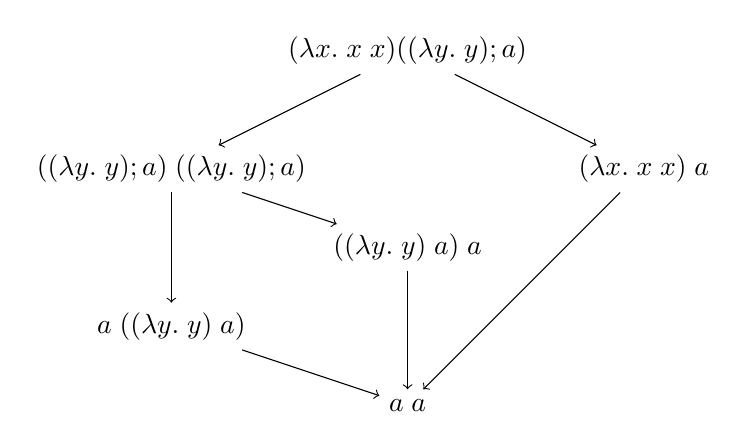
\begin{tikzpicture}
    \node(T1) at ( 0,  0) {$(\lambda x.\; x\;x)((\lambda y.\;y); a)$};
    \node(T2) at (-3, -1.5) {$((\lambda y.\;y); a)\;((\lambda y.\;y); a)$};
    \node(T3) at ( 3, -1.5) {$(\lambda x.\; x\;x)\;a$};
    \node(T4) at ( 0, -2.5) {$((\lambda y.\;y)\; a)\;a$};
    \node(T5) at (-3, -3.5) {$a\;((\lambda y.\;y)\;a)$};
    \node(T6) at ( 0, -4.5) {$a\;a$};

    \draw[->] (T1) edge (T2) (T2) edge (T4) (T4) edge (T6) (T3) edge (T6)
              (T2) edge (T5) (T5) edge (T6) (T1) edge (T3);
  \end{tikzpicture}
  \end{center}

  This raises the questions : \begin{itemize}
    \item Are some paths better than others ?
    \item Is there always a result in the ? Is it unique ?
  \end{itemize}

  \subsection{Normalization}

  \subsection{Reduction strategies}

  \subsection{Confluence}

\end{document}
